%% This is an example first chapter.  You should put chapter/appendix that you
%% write into a separate file, and add a line \include{yourfilename} to
%% main.tex, where `yourfilename.tex' is the name of the chapter/appendix file.
%% You can process specific files by typing their names in at the 
%% \files=
%% prompt when you run the file main.tex through LaTeX.
\chapter{Introduction}

Modeling is a game of balance. Tractability and reasonable solution times fight against the physical realities of vast length and time scales. The assumptions one makes when formulating a model directly impact the solution methods that can be brought to bare to the problem at hand. There is almost always guaranteed trade-offs between the level of simplification of a model and the amount of time needed to solve that model.

Granular media present an interesting intermediary between the world of the discrete and continuum. While often times they are studied in contexts where continuum approximations are appropriate (i.e. geological), their behavior at much smaller length scales (a bucket of sand at the beach or flow through an hour glass) are still of great interest. However at those more everyday scales, the length scale of a single grain of sand is a relatively large proportion of the scale of the entire problem, and thus cannot be ignored. And even at the larger aforementioned geological scales, the initiation of an earthquake, for an example, still relies on individual grains of sand slipping and deforming against each other.

The great challenge, then, is to formulate a model that can capture length scale effects but still have enough simplifying assumptions to make the problem solvable with efficient methods. This however seems to fly in the face of the modeling trade-off previously discussed; it is nearly impossible to have a single model that allows for fine-scale resolution and yet ignores those small length scales to become efficiently solvable. The solution we now propose addresses this issue by ignoring the "single" part of the "single model" clause, and instead hybridizes two distinct models to yield the two distinct attributes desired: resolution of length scale while maintaining efficient solvability. It is noted that the current work focuses on cohesionless granular systems, and thus approximate dry granular systems with no sources of attraction, like liquid bridges or electrostatic charges.

The work is structured as follows. The remainder of chapter 1 puts the current work in the greater academic context and discusses prior work on the modeling of granular media. Hybridization models in and out of granular media contexts are also discussed. 

Chapter 2 discusses the discrete element method used and some details of its algorithmic solution. While the level of detail presented may seem overly exhaustive, it provides important context for where the hybridization technique interfaces with the discrete element method.

Chapter 3 discusses the continuum models used. The method used to solve these models, the Material Point Method, is also discussed in detail.

Chapter 4 introduces the hybridization technique. Its goal, formulation, and solution are discussed.

Chapter 5 shows examples of the hybridization technique at work, with comparisons to the discrete and continuum model solutions, as well as to literature.

Chapter 6 builds off of the work shown in the previous sections, and introduces new enrichment schemes that are needed for problems beyond the ones discussed in Chapter 5.

Finally chapter 7 concludes the thesis and discusses future work. 

\section{Granular Media Modeling}

The ubiquity of granular media in everyday life cannot be understated. We walk on it on trails, drive over it on roads \cite{sullivan06}, ingest it in our pharmaceuticals, and eat it in our meals. Slightly less directly, granular media is second only to water for the type of material most commonly handled in industry \cite{Richard:2005:Slow}. Granular materials also appear often in the context of special effects in visual media. CGI scenes at a beach or dessert require realistic simulation of granular media, and the most straightforward way to do this is to solve physically realistic models for granular behavior. Despite this ubiquity however, a comprehensive model that can capture the behavior of granular media remains elusive. 

\begin{figure}[htp] 
    \centering
    \subfloat[data a]{%
        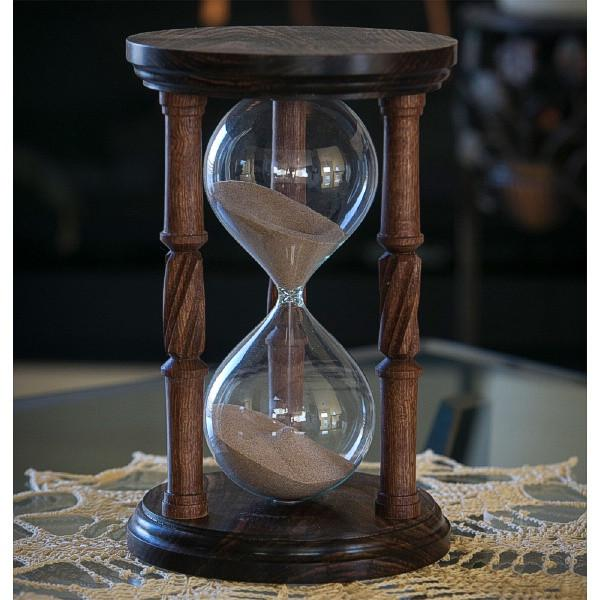
\includegraphics[width=0.4\textwidth]{figs/hourglass_whole.jpg}%
        \label{fig:a}%
        }%
    \hfill%
    \subfloat[data b]{%
        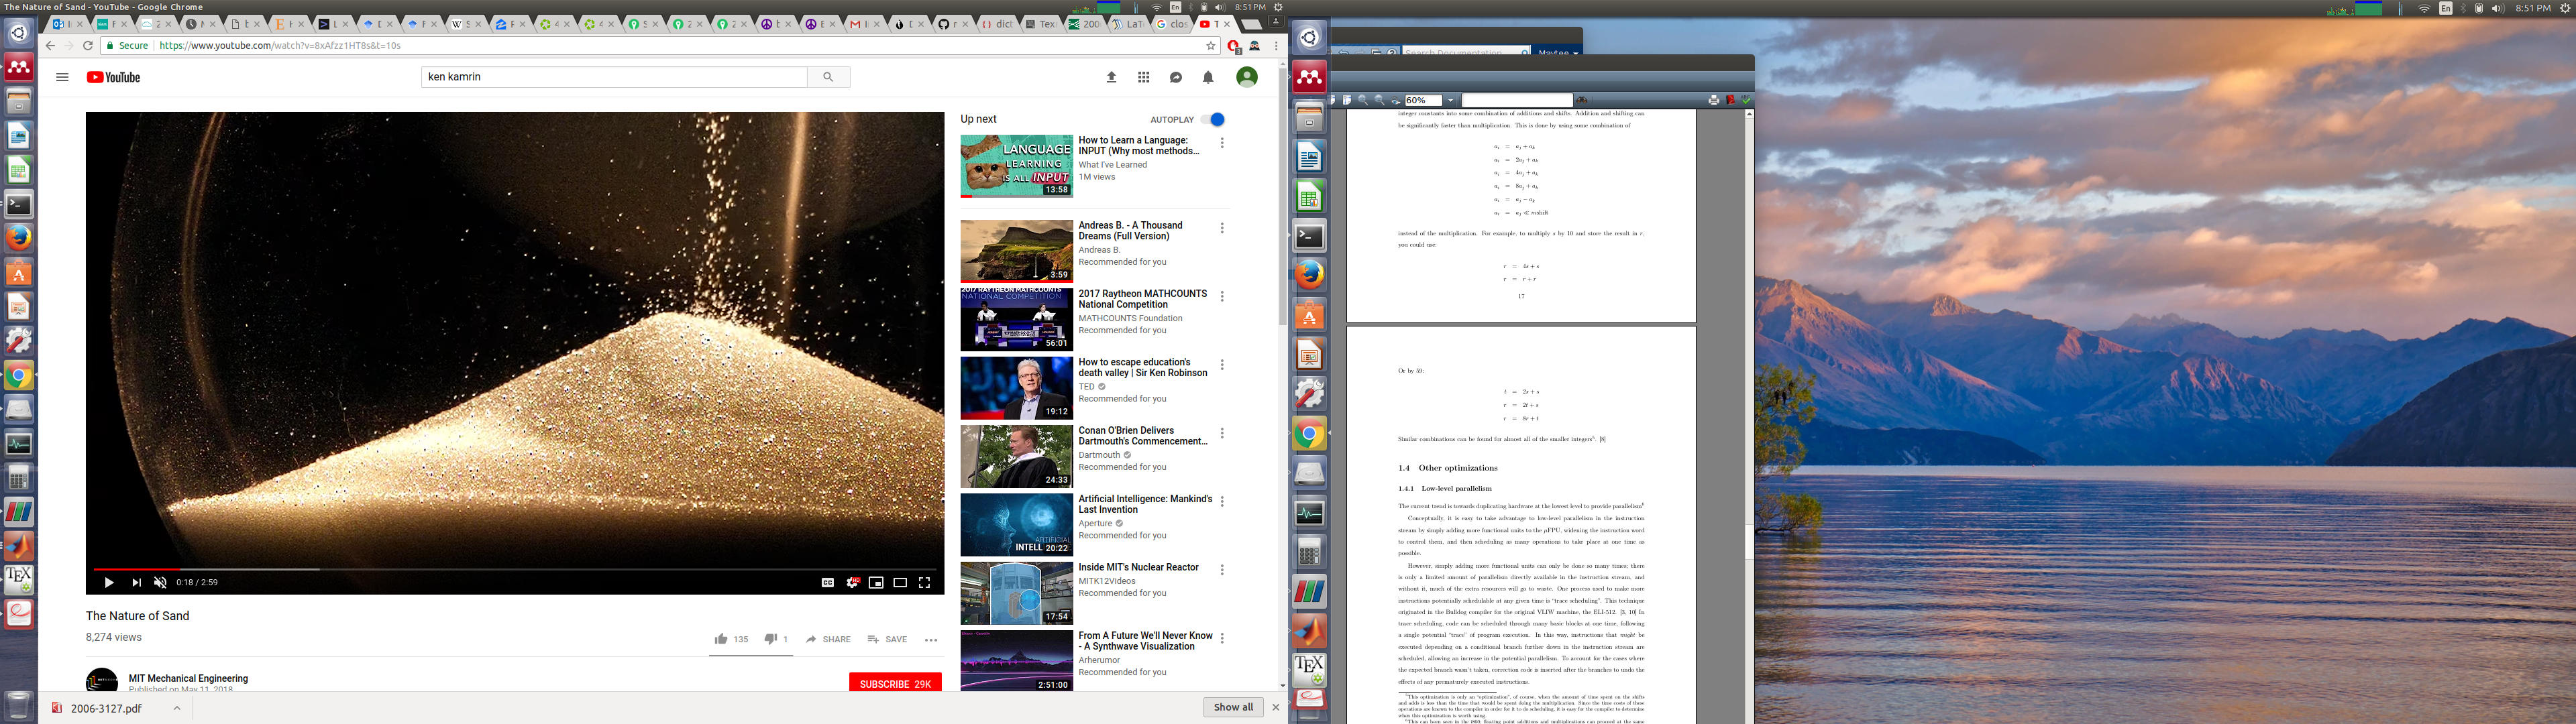
\includegraphics[width=0.4\textwidth]{figs/hourglass_closeup.png}%
        \label{fig:b}%
        }%
    \caption{Flowing hourglass displaying three distinct phases, with entire hourglass 			(a) and closeup of bottom region (b)}
    \label{hourglass}
\end{figure}

While much of the difficulty stems from the length and time scale problems mentioned before, granular media is also unique from many other materials in its ability to transition between different states. This is clearly evident in a flowing hourglass, as shown in Figure \ref{hourglass}. At the bottom of the hourglass, settled sand acts as a solid, able to support compressive stress without flowing. At the top of the static pile is a region of grains flowing over the static region, acting like a liquid. In between the top and bottom of the hourglass the grains flow much like a dilute gas, with no cohesive structure and interacting via collisions.

Different models and solution techniques are able to capture granular behavior in a given state, though of course with trade-offs in accurately capturing behavior in other states. A summary of different methods are discussed. 

\subsection{Discrete Methods}
Perhaps the most straightforward way one could model a system of granular material is to model the grains themselves. Methods that model individual grains and the interactions between them fall under the umbrella of discrete methods. While this can be expensive for very large systems (greater than approximately 50,000 particles per core given current CPU capabilities), the one-to-one correspondence of a single simulated grain to a physical grain can produce accurate results. Discrete element methods can largely be broken down into two classes: penalty based methods and contact dynamics.

Penalty methods, as their names suggest, penalize the overlap of particles with some type of force that is a function of that overlap. The discrete element method (note that in some literature the term "discrete element method" is used to denote the larger class of what is here termed "discrete methods"), first formulated by Cundall and Strack, still enjoys much use due to its simplicity and accuracy \cite{Cundall:1979}. Even within the confines of the simplicity of the proposed method though, great generalizability can be realized by having a free choice of the penalty function. The advantages of course come at some cost. For example, a major drawback is that, depending on the choice of penalty function, multiple material parameters may need to be fit to experiment. The material parameters themselves may then put constraints on the computational solve time. To concretely demonstrate this point, many penalty models have some notion of an elastic parameter that must be tuned. However, most individual grains of sand are fairly stiff, with \textcolor{red}{FINDREFERENCE} bulk moduli on the order of $49 GPa$ and densities on the order of $2000 kg/m^3$. These properties, combined with the small size of many grains (~0.1 mm in diameter), result in a large wave speed through the material that travels a small distance, and this must be resolved within a given time step. Implicit methods of course exist to alleviate this issue somewhat, but those come with the usual drawbacks of additional computational overhead elsewhere.

Contact dynamics on the other hand treats grains as completely rigid and allow no overlaps. They are then formulated as optimization problems, and more specifically, mixed linear complementarity formulations, minimizing some potential with a no overlap constraint. While the question of material properties is then largely avoided in these methods, the introduction of friction and other properties is much less straightforward than in the formulation of discrete element methods. The lack of material properties is also a double-edged sword of sorts, as while infinitely stiff grains are often a better approximation of a system of grains than computational grains that are extremely soft, the reality is that grains do have a finite, though large, stiffness. Capturing that finite stiffness and its consequences, such as a finite wave speed and non-negligible grain deformation, can be crucial in some applications. These properties are in fact important for the hybrid scheme, and will be discussed later.

A key characteristic of both classes of discrete methods is that they can easily capture all phases of discrete matter. If compressed by exterior forces or boundaries, they act like a solid, able to support load through the creation of force chains, much like physical granular media. The removal of these forces and boundaries, and/or the introduction of shear forces, causes grains to flow over other grains in a liquid-like fashion. Pouring a system of discrete grains will see the grains separate, capturing a granular gas.

Another property of discrete element methods is that they are able to elucidate particle level properties and dynamics that are difficult to gather from experiment. Photoelastic disks can be used to investigate force chains, such as in the pioneering work of Behringer et al and continued by the likes of Daniels et al \textcolor{red}{FINDREFERENCE}. However these photoelastic disks are made of relatively soft polymers and are mostly used to investigate 2D arrangements of disks, and not 3D arrangements of spheres. On the other hand, discrete element methods calculate inter-particle forces out of necessity and can thus report quantitative data for these contacts. Expanding from 2D to 3D is also a straightforward process, and every contact in a 3D system can be easily obtained. The dynamics of every single grain in a system modeled with discrete methods can also be tracked and studied, which can be done in experiment, but only with much difficulty and cost, i.e. methods such as X-ray tomography and CT scans \textcolor{red}{FINDREFERENCE}. While computational expenses can limit the size of simulated systems, physical limitations of scanning equipment can limit the size of an experimental system that can be studied, greatly hampering one of the key advantages of experiments over simulations in granular media: scale. 

Thus despite the drawbacks of discrete element methods, they are still popular and widely used in congruence with, and sometimes in the place of, physical experiment. The ability to accurately capture grain-scale level dynamics, and to obtain quantitative data for every grain and contact, means that they can effectively be treated as computational "ground truth" for simulated granular systems. When accuracy in a simulation is needed, discrete element methods can be used with confidence, at least compared with other methods.

\subsection{Continuum Models}
\begin{figure}[htp] 
    \centering
    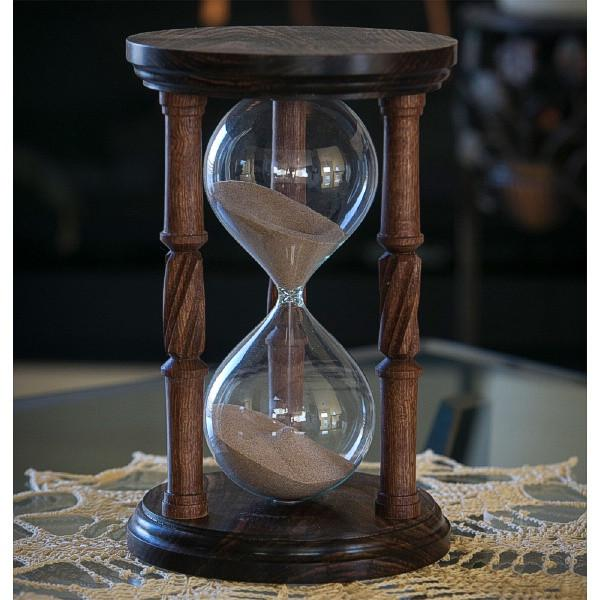
\includegraphics[width=0.4\textwidth]{figs/hourglass_whole.jpg}
    \caption{Aftermath of a landslide in La Conchita California.}
    \label{landslide}
\end{figure}

As stated before, for large (what constitutes "large" varies from system to system, though ~20 grain diameters per continuum element dimension is used as a rule of thumb \textcolor{red}{FINDREFERENCE}) granular systems, one can ignore the fact that there are individual grains of sand, treat the system as a continuous granular medium, and retain many physical properties of the system. A classic example of this can be seen in Figure \ref{landslide}, which shows the aftermath of a landslide. A useful feature of the shown landslide is that a road can be seen that cuts through the hill, and acts as a deformation marker. The deformed shape is reminiscent of Poiseuille flow, suggesting that the moving bulk is well represented by a continuum.

Continuum theory applied to granular media in fact goes back more than 50 years, with the pioneering work of Coulomb who proposed a relation between shear stress, pressure, and a coefficient of friction in a granular continuua, very similar in form to Coulomb friction \textcolor{red}{FINDREFERENCE}. Since that initial proposal, granular continuum theory has been greatly expanded upon. The incorporation of additional complexity displayed in physical granular systems into the continuum theory have resulted in models that capture behavior such as critical-state, and anisotropy \cite{Schofield:1968:Critical}\cite{Dafalias:2004:Sand}.

Much work on granular continuum theory has been conducted in the fields of civil engineering and soil mechanics, where understanding the behavior of granular systems under load is crucial \textcolor{red}{FINDREFERENCE}. There is thus a large body of work on granular media in a solid phase, and continuum modeling of grains in this state is well understood. Granular gases too have been well investigated, with kinetic theory being effectively used to understand granular systems in this state.

The "liquid" flowing phase of granular materials has been much more difficult to model. It was only recently that a seminal study conducted by GDR MiDi suggested a possible model for flowing granular systems \cite{Midi:2004:Dense}. The rheological model posited, commonly referred to as the $\mu(I)$ relation ($\mu$ of I), suggests a yield condition similar to that suggested by Coulomb nearly half a century ago, but with a friction coefficient dependent on a nondimensional inertial number, $I$, which describes the ratio of inertia to confining pressures in a granular system. Further work by Jop and De Cruz provided empirical relations between the friction coefficient $mu$ and $I$ \cite{Jop:2006:Constitutive}\textcolor{red}{FINDREFERENCE}. Further extensions of this model have since been proposed, and work continues to this day on clarifying the high and low inertia number bounds of the $mu(I)$ relation. 

All of the previously described models, while increasingly complex, still retain some simplicity in the sense that they are all local models. No length-scale is introduced, and thus no non-local effects are captured. This deficiency has been recently addressed by the work of Kamrin et al, who have proposed a non-local continuum model and thus introduce a notion of a length scale back into the continuum model \cite{Kamrin:2012:Nonlocal}. At first glance this seems provides a possible solution to the beginning stated problem of capturing length-scale effects while retaining the ability of efficient continuum equation solving methods. However, much additional work must be done to completely characterize these non-local models, and thus for now cannot be relied upon to have the fidelity of discrete methods which capture length-scale effects by their very nature.

\subsection{Related Hybridization Work}
Quasi-Continuum and Arlequin-type methods have been
explored primarily for crystalline solids, to expedite otherwise lengthy atomistic simulations by hybridizing with a
crystal plasticity continuum model in zones where atomistic refinement is not
needed~\cite{Tadmor:1996,Smith:2001,Shimokawa:2007,Zhang:2005,Dhia:1998}. The idea of hybridizing discrete-particle and
continuum approaches to simulate granular media is in its infancy, with only initial work done to show the validity of
communicating mechanics between discrete grains and finite-element representations~\cite{Yan:2010}. Recent work has explored when
continuum and discrete treatments are simultaneously accurate \cite{Rycroft:2009,Kamrin:2010,Kamrin:2014}, including an
Arlequin-type method that couples statically-defined regions of a discrete element (DEM) simulation to the interior of a continuum
FEM-based simulation to enrich stress fields around drill tips, for instance \cite{Wellmann:2012}. We build on and extend these ideas to
target regimes in which enriched degrees of freedom are required at surfaces, and where the boundary between continuum
and discrete regimes evolves dynamically.

In the granular physics and graphics literature, lower-level ideas have been tried where instead of implementing a
general continuum model, the user imposes kinematic constraints to the particle motion in certain regions, often chosen
based on experience with the problem at hand. The graphics literature has explored freezing rigid bodies that are
sufficiently stationary~\cite{Smith:2005}. Similar techniques have been proposed to accelerate the generation of
granular packings for industrial applications~\cite{Mio:2009}. In common granular setups such as rotating tumblers and
growing sand piles, semi-empirical models can be used to guess zones of rigid material, and grains in these zones can be
removed from the discrete update \cite{McCarthy:1998,Hsu:2010,Zhu:2010,Bouchaud:1994}. Holladay et al.\cite{Holladay:2012}
carve out interior regions of granular materials moving at constant velocities and replace these groups of grains with
meshes, but this method does not homogenize over rigidly rotating regions or over shear flows, and as the paper notes,
can lead to volume loss. These ideas have been developed further in follow-up work ~\cite{Holladay:2013,Munns:2015}.
These methods make no claims as to the accuracy of the techniques for science and engineering applications, and have not
yet demonstrated stable granular flows.
